\section{Experimental Evaluation}
\label{s4-experiments}

In this section, we (1) benchmark gigaFLOPS enhanced version of the variable-size
batched matrix inversion routine based on GJE; (2)
analyze the performance of the complete block-Jacobi preconditioner (generation
and application); and
(3)
assess the efficiency of block-Jacobi preconditioning in an iterative solver
setting.

We begin by comparing the new BGJE kernel against the
version presented in~\cite{Anzt:2017:BGE:3026937.3026940} and against two batched
inversion routines available in NVIDIA's cuBLAS library: \textcolor{black}{{\tt
getriBatched} and {\tt matinvBatched}}. We note that both
\textcolor{black}{cuBLAS routines} can only operate on batches of problems where
all matrices are of the same size.

Next, to evaluate the the performance benefits for the block-Jacobi
preconditioner generation stage, in isolation, we combine our variable-size BGJE
routines with the improved extraction and insertion procedures, and we test the
block-inverse generation for different sparsity structures and block sizes. For
this purpose, we consider a set of test matrices from the SuiteSparse Matrix
Collection\footnote{Visit
	\url{http://www.cise.ufl.edu/research/sparse/matrices/}.} (formerly known as the
University of Florida Sparse Matrix Collection).
In addition to the preconditioner generation, we also compare the specialized
block-Jacobi application kernel based on variable-size batched {\sc gemv} with
the generic {\sc spmv} routine from MAGMA-sparse~\cite{magma}.

Finally, to analyze the practical effects of the block-Jacobi preconditioning on
an iterative solver, we integrate the block-Jacobi preconditioner into an Induced 
Dimension Reduction Krylov solver with shadow space dimension 4 (~IDR(4)~) and demonstrate the time-to-solution 
improvements obtained by replacing a scalar-Jacobi preconditioner with a 
block-Jacobi variant.

\subsection{Hardware and software framework}

For the experiments, we use the two most recent NVIDIA GPU architectures, which have full
support for double-precision computations: the Kepler K40 (Compute Capability
3.5)
and the Pascal P100 (Compute Capability 6.0).
We do not consider the older
Fermi and Maxwell architectures, as the former lacks support for warp shuffle
instructions, and the latter does not implement full double-precision support.
Because the batched matrix inversion routines, the block-Jacobi generation kernel,
and the iterative solvers proceed exclusively on the GPU, details about the node's
broader hardware specifications are irrelevant in the following experiments.

Our kernels are implemented using CUDA 8.0 and are designed to be integrated
into the MAGMA-sparse library~\cite{magma}. MAGMA-sparse also provides the
testing environment, the block-pattern generation, and the sparse solvers used
in our experiments. All computations use double-precision arithmetic---the
standard in linear algebra.

\begin{figure*}
\begin{center}
{\scriptsize
\begin{tabular}{cc}
K40 & P100\\
\hline
\multicolumn{2}{c}{Problem size 32}\\
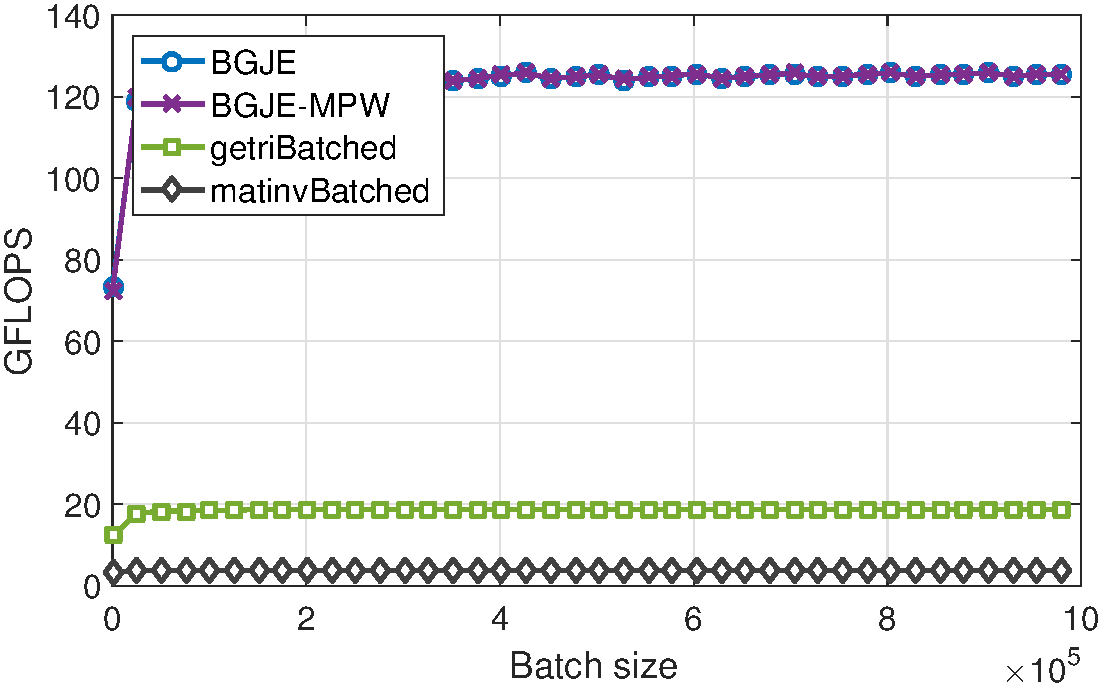
\includegraphics[width=.46\columnwidth]{plots/gje_n_d_K40_32.pdf}&
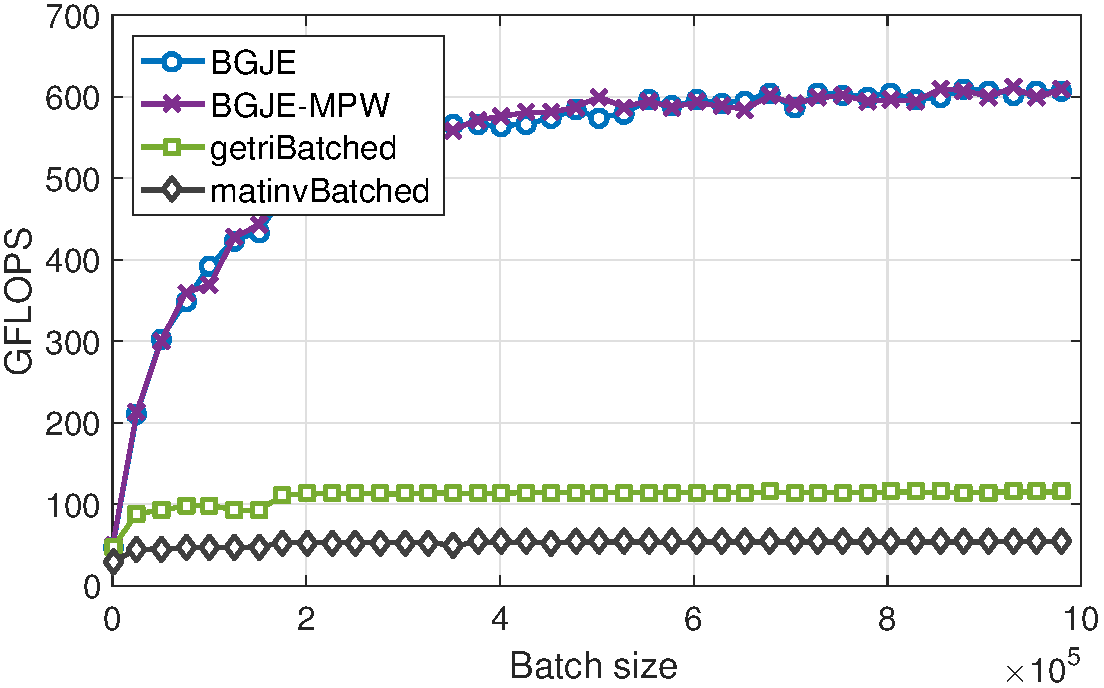
\includegraphics[width=.46\columnwidth]{plots/gje_n_d_P100_32.pdf}\\
\hline
\multicolumn{2}{c}{Problem size 16}\\
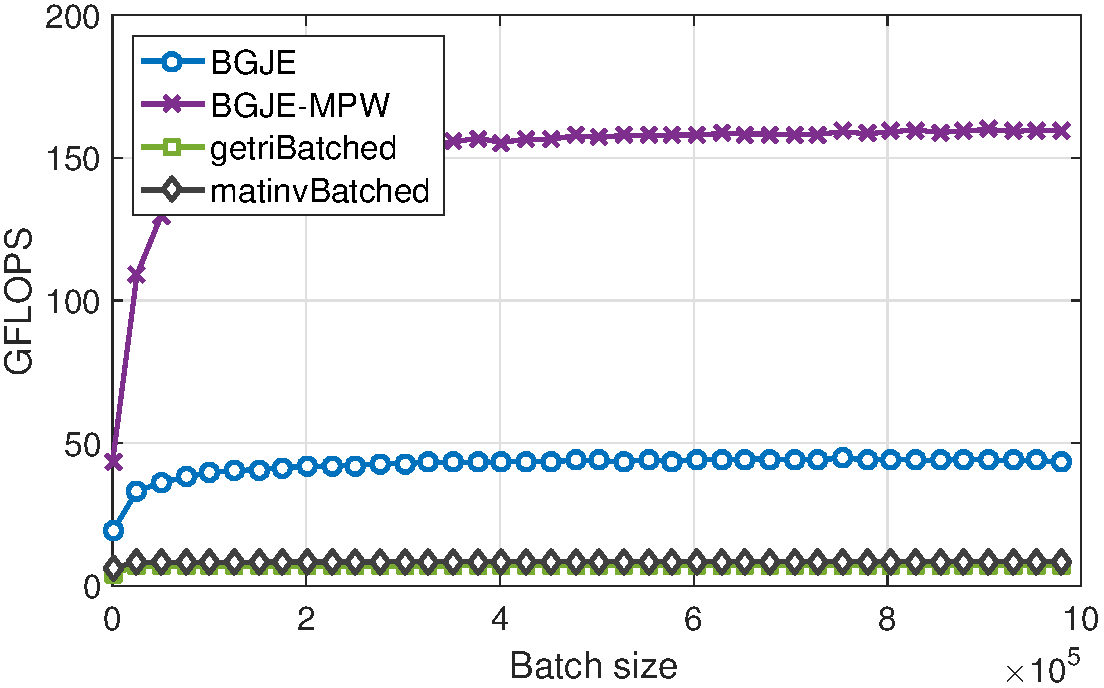
\includegraphics[width=.46\columnwidth]{plots/gje_n_d_K40_16.pdf}&
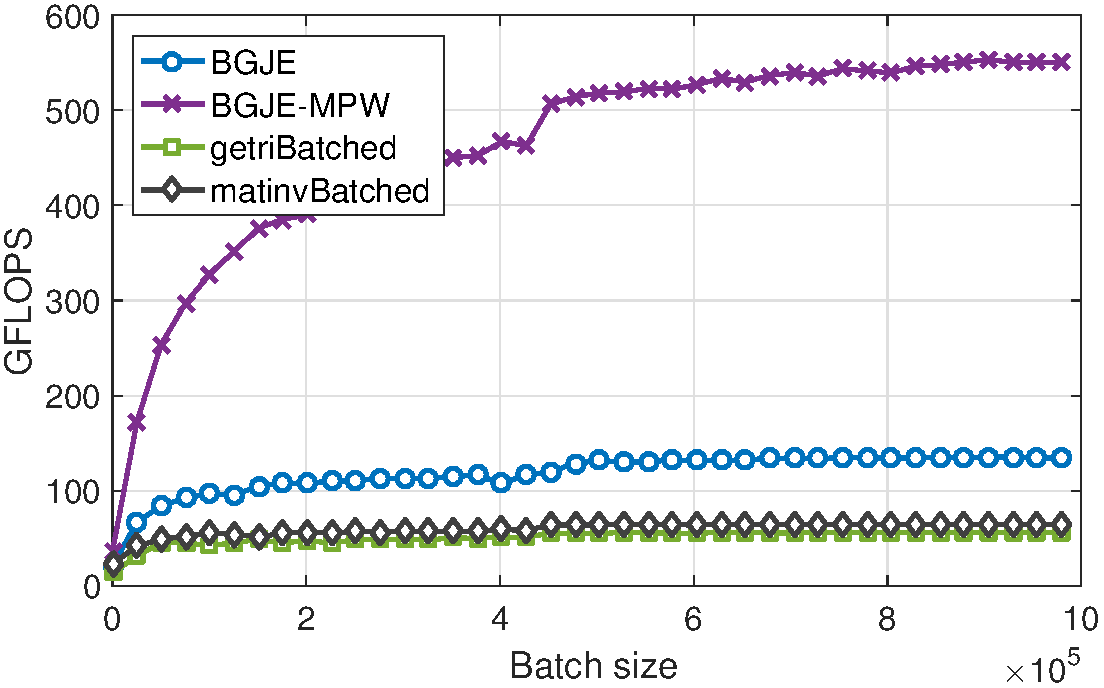
\includegraphics[width=.46\columnwidth]{plots/gje_n_d_P100_16.pdf}
\end{tabular}
}
\end{center}
\caption{
Performance comparison of batched matrix inversion routines for various batch sizes. 
Top row shows matrices of size 32 $\times$ 32 and the bottom row shows matrices of size 16 $\times$ 16.
}
\label{fig:bgje-mpw-performance}
\end{figure*}

\begin{figure*}
\begin{center}
{\scriptsize
\begin{tabular}{cc}
K40 & P100\\
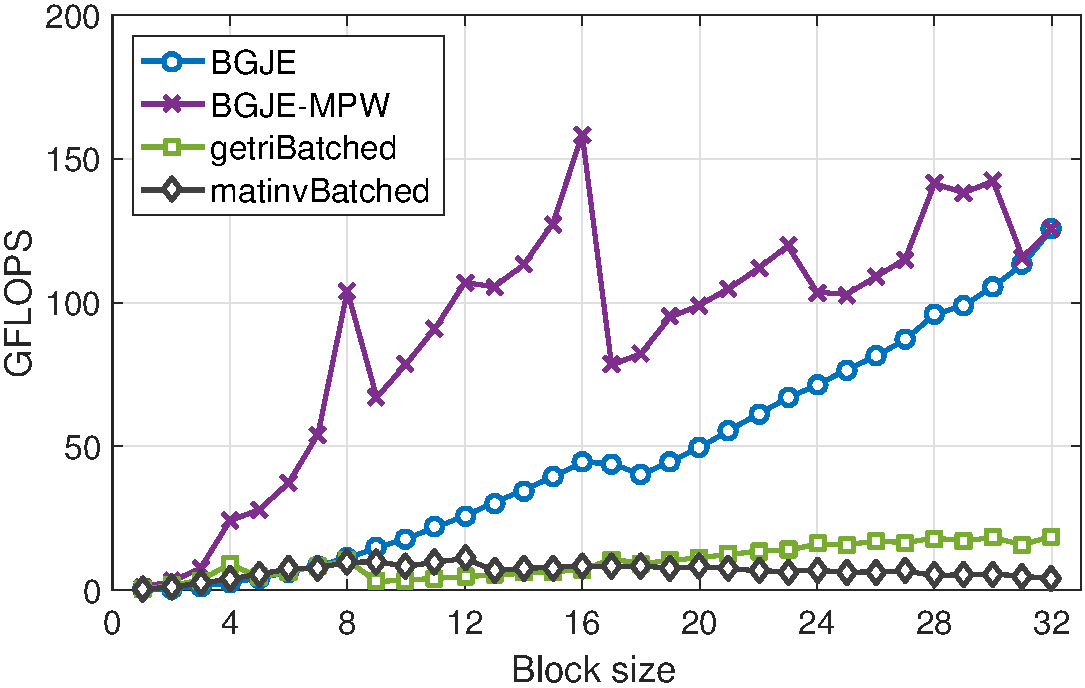
\includegraphics[width=.46\columnwidth]{plots/gje_bs_n_d_K40.pdf}
&
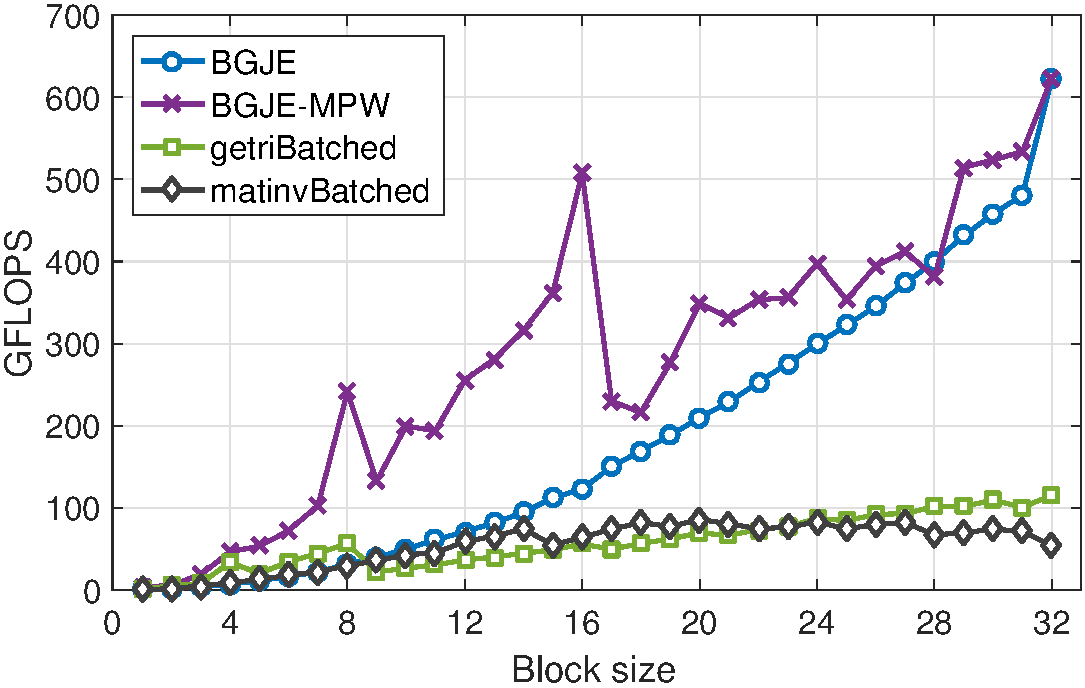
\includegraphics[width=.46\columnwidth]{plots/gje_bs_n_d_P100.pdf}
\end{tabular}
}
\end{center}
\caption{%
Performance comparison of batched matrix inversion routines
    for various matrix sizes.}
\label{fig:bgje-mpw-fixed-batch}
\end{figure*}

\subsection{Batched matrix inversion}

This section analyzes the performance of four batched routines for matrix
inversion on GPUs; {\tt BGJE}, {\tt BGJE-MPW}, {\tt getriBatched}, and {\tt matinvBatched}.
\begin{enumerate}
\item
\textbf{\tt BGJE} is the variable-size BGJE inversion kernel from~\cite{Anzt:2017:BGE:3026937.3026940}.
\item
\textbf{\tt BGJE-MPW} is the enhanced kernel that
       incorporates the BGJE improvements described in this paper.
\item
\textbf{\tt getriBatched} renders the batched matrix inversion using two
functions from NVIDIA's cuBLAS library: (1) \texttt{\tt getrfBatched} computes
the LU factorization of the matrix batch, then (2) \texttt{\tt getriBatched}
obtains the inverses using the results of the previous routine. All matrices in
the batch are required to be of the same size.
\item
\textbf{\tt matinvBatched} is NVIDIA's
routine that merges the two calls of the {\tt getriBatched} routine into
a single kernel. Its functionality is limited to operating on batches of
equal-size matrices with an upper bound of 32 $\times$ 32.
\end{enumerate}

We note that the scope of the distinct batched inversion routines is slightly
different: {\tt BGJE}, {\sc BGJE-MPW}, and {\tt matinvBatched} only support
matrices of size up to 32 $\times$ 32; and neither {\tt matinvBatched} nor {\tt
	getriBatched} support batches containing matrices of different sizes. Therefore,
we limit the performance comparison to batches composed of equal-size matrices
of up to 32 $\times$ 32. While this upper bound is usually not a problem in the
context of block-Jacobi preconditioning, handling batches that contain variable-size 
matrices is essential to accommodating the inherent block structure of FEM
discretizations. Consequently, the cuBLAS routines will not be considered
in the complete preconditioner generation and application experiments.

Figure~\ref{fig:bgje-mpw-performance} compares the performance, in terms of
gigaFLOPS (billions of arithmetic floating-point operations per second), for two 
fixed matrix sizes (32 $\times$ 32 and 16 $\times$ 16) while increasing the matrix count (batch size).
In a case where the matrix order is 32, both {\tt BGJE} and {\tt BGJE-MPW} deliver the
same performance because, in this scenario, {\tt BGJE-MPW} also schedules a single
problem per warp. For this matrix size, the performance of both variable-size
BGJE routines exceeds 600 gigaFLOPS {(13\% of the theoretical peak)} on P100 and
around 125 gigaFLOPS {(9\% of peak)} on K40. These rates correspond to a 6$\times$
speedup over the batched inversion using {\tt getriBatched}, and at least a
12$\times$ speedup over {\tt matinvBatched}.

The older K40 architecture has a significantly lower register-per-core ratio
compared to the P100. Because our {\tt BGJE} and {\tt BGJE-MPW} routines make heavy
use of registers, a reduced register count limits the number of threads/warps
that can be active on a multiprocessor, which explains the large performance gap
between the K40 and P100 GPUs.

The two graphs on the left side of Figure~\ref{fig:bgje-mpw-performance} clearly show 
that the registers are indeed a performance bottleneck on the K40. 
For batched problems consisting of 16 $\times$ 16 matrices, each thread only utilizes 
16 registers (instead of 32 registers for 32 $\times$ 32 matrices), allowing more active 
threads---and therefore more active warps---per
multiprocessor. As a result, the {\tt BGJE-MPW} kernel delivers about 160~gigaFLOPS
for the smaller matrix sizes but only around 125~gigaFLOPS for the larger matrices. In
comparison, the {\tt BGJE} kernel, which can only handle a single problem per
warp, achieves a scant 40~gigaFLOPS for the small case. Moreover, both cuBLAS
batched inversion routines, {\tt getriBatched} and {\tt matinvBatched}, deliver
a meager 8~gigaFLOPS for this problem.

Again, note that the {\tt BGJE} kernel pads the matrices with dummy
elements to size 32~$\times$~32 and inverts one system per warp. On the P100, this
delivers less than 150~gigaFLOPS for a batch composed of matrices of size 16~$\times$~16. 
In contrast, the performance of the {\tt BGJE-MPW} routine exceeds 550~gigaFLOPS in similar conditions.
Thus, although the performance of {\tt BGJE-MPW} is lower for a 16~$\times$~16 matrix
than for a 32~$\times$~32 matrix (which was expected because the
data-movement-to-floating-point-operation ratio grows with the matrix
size), {\tt BGJE-MPW} is about one order of magnitude faster than the matrix
inversion functions provided in NVIDIA's cuBLAS.

A detailed analysis for different matrix sizes is given in
Figure~\ref{fig:bgje-mpw-fixed-batch}. In this experiment we fixed the batch
size to 500,000 matrix problems and varied the dimension of the matrices in the
batch from 1~$\times$~1 to 32~$\times$~32. For both architectures, {\tt BGJE} exhibits a superlinear
performance drop as the matrix size is reduced. This is because,
for a batch with matrices of size $k$, each warp performs $2k^3$ useful
operations, while the total volume of operations (including those on dummy data
used for padding) is $2k \times 32^2$. In contrast, {\tt BGJE-MPW} avoids most
dummy operations and experiences only a linear performance loss---owing to
inactive threads---between consecutive powers of two. Peaks for 16~$\times$~16 matrices and
8~$\times$~8 matrices clearly mark the thresholds where multiple small problems can be handled by a
single warp without introducing any computational overhead. The performance
lines for {\tt BGJE-MPW} are more erratic than those observed for the other
routines. The reason is that {\tt BGJE-MPW} is implemented using C++ templates
to generate a specialized version of the kernel for each matrix size. While this
approach succeeds in minimizing the register count and the number of operations
performed by the size-specific kernels, the kernel-specific resource
requirements impact the number of warps that are active per multiprocessor and,
ultimately, the kernel-specific performance.

\begin{figure}
\begin{center}
{\scriptsize
\begin{tabular}{c}
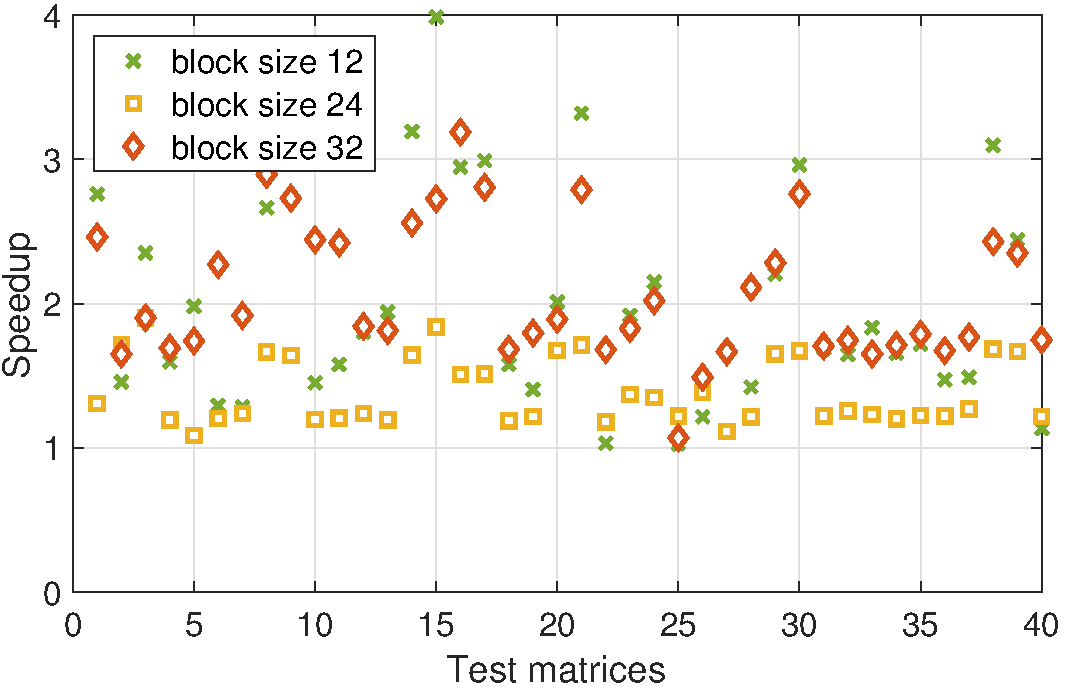
\includegraphics[width=.48\columnwidth]{plots/shared_mem_improvement.pdf}
\end{tabular}
}
\end{center}
\caption{
Performance improvement from reducing the shared memory size in the 
block-Jacobi generation using shared extraction/insertion.
}
\label{fig:reducedshared}
\end{figure}
\subsection{Block-Jacobi generation}


We now turn our attention to the complete block-inversion procedure that
produces the block-Jacobi preconditioner. This includes the extraction of the
diagonal blocks from a sparse data structure, followed by the explicit
inversion, and then the insertion of the inverse blocks into the preconditioner
matrix. As previously mentioned, the routines are ``merged'' into a single CUDA
kernel that performs all three steps: (1) extraction from the sparse matrix
structure, (2) inversion, and (3) insertion into the sparse preconditioner matrix. In
this subsection, we compare three strategies for the generation of the
block-Jacobi preconditioner, with the first strategy corresponding to an
implementation that was already proposed
in~\cite{Anzt:2017:BGE:3026937.3026940}, and the last two strategies realizing the
improvements described in section~\ref{sec:s3-kernel}:
\begin{enumerate}
    \item {\sc cached}: cached extraction/insertion with {\tt BGJE};
    \item {\sc shared}: shared extraction/insertion with {\tt BGJE}; and
    \item {\sc shared-mpw}: shared extraction/insertion with {\tt BGJE-MPW}.
\end{enumerate}
Both {\sc shared} and {\sc shared-mpw} use the reduced memory shared extraction
described in subsection~\ref{subsec:s3-extraction}.  
{
Figure~\ref{fig:reducedshared} reveals that reducing the shared memory in the 
{\sc shared} strategy can make the block-Jacobi generation up to four times 
faster. The problem-specific benefits depend on the the upper bound for the 
block size, the pattern of the system matrix determining the actual size of the 
distinct diagonal blocks, and the hardware characteristics determining how many 
thread blocks a multiprocessor can schedule in parallel.}



\begin{figure*}
\begin{center}
{\scriptsize
\begin{tabular}{cccc}
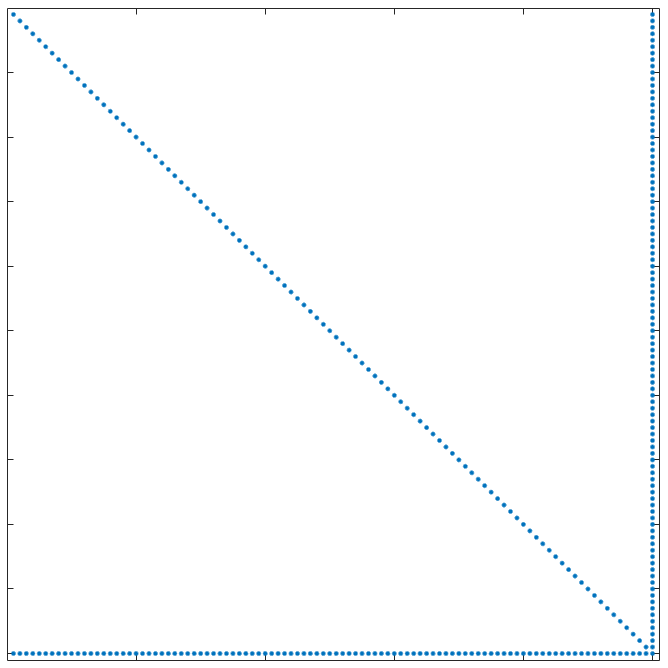
\includegraphics[width=.2\columnwidth]{plots/arr.png}
&
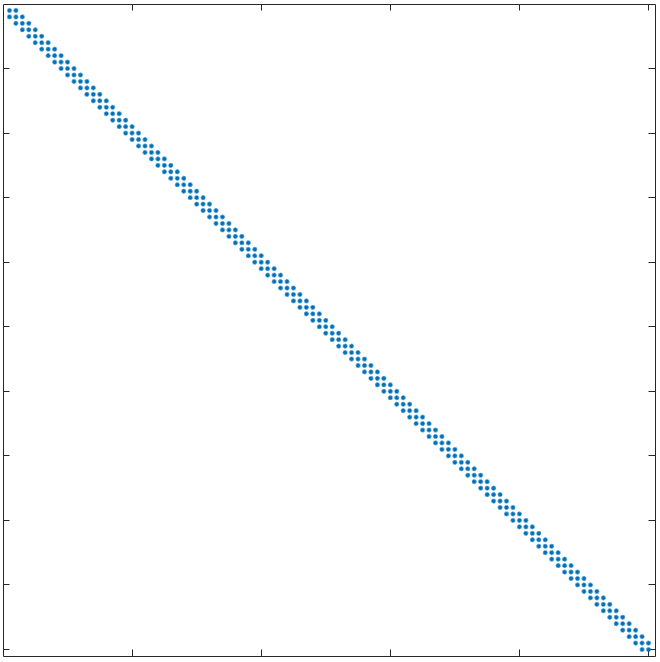
\includegraphics[width=.2\columnwidth]{plots/tdg.png}
&
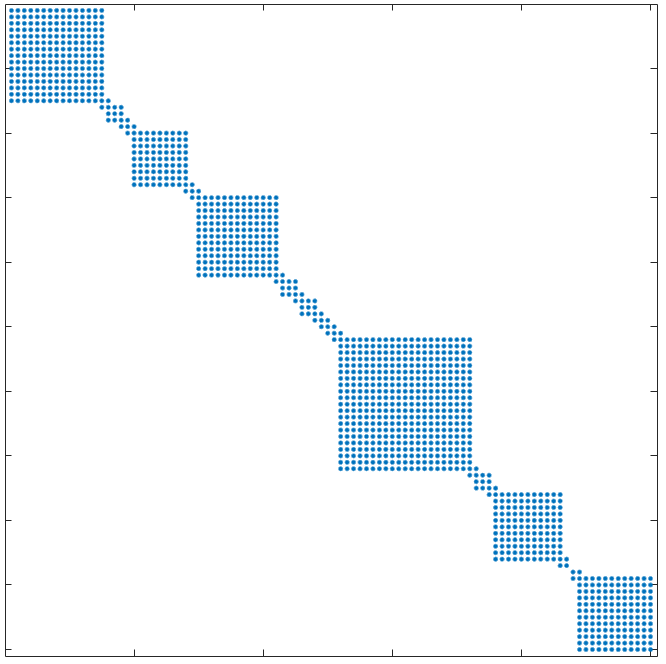
\includegraphics[width=.2\columnwidth]{plots/rnd.png}
&
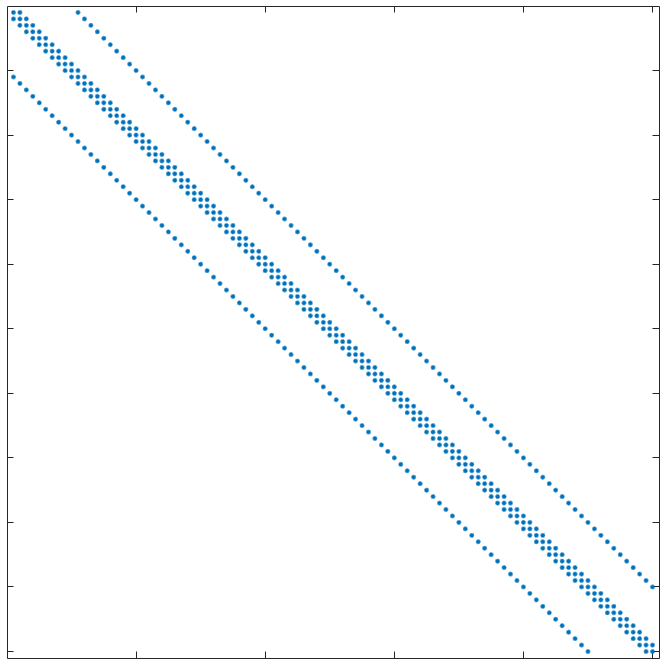
\includegraphics[width=.2\columnwidth]{plots/lap.png} \\
Arrow structure & Tridiagonal structure & Random block struct. & Laplace structure
\end{tabular}
}
\end{center}
\caption{%
Sparsity plots of test matrices used to evaluate the diagonal block extraction.%
}
\label{fig:sparsityplots}
\end{figure*}


\begin{figure*}
\begin{center}
{\scriptsize
\begin{tabular}{cc}
K40 & P100\\
\hline
\multicolumn{2}{c}{Arrow structure}\\
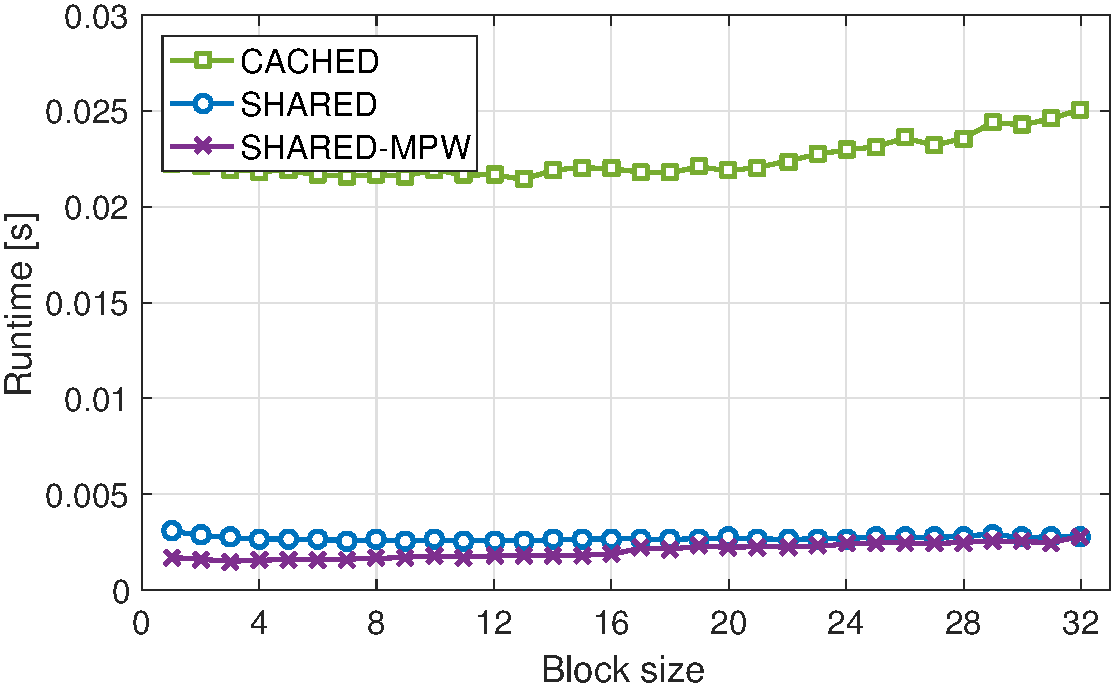
\includegraphics[width=.46\columnwidth]{plots/ARR_bjp_setup_bs_d_K40.pdf}
&
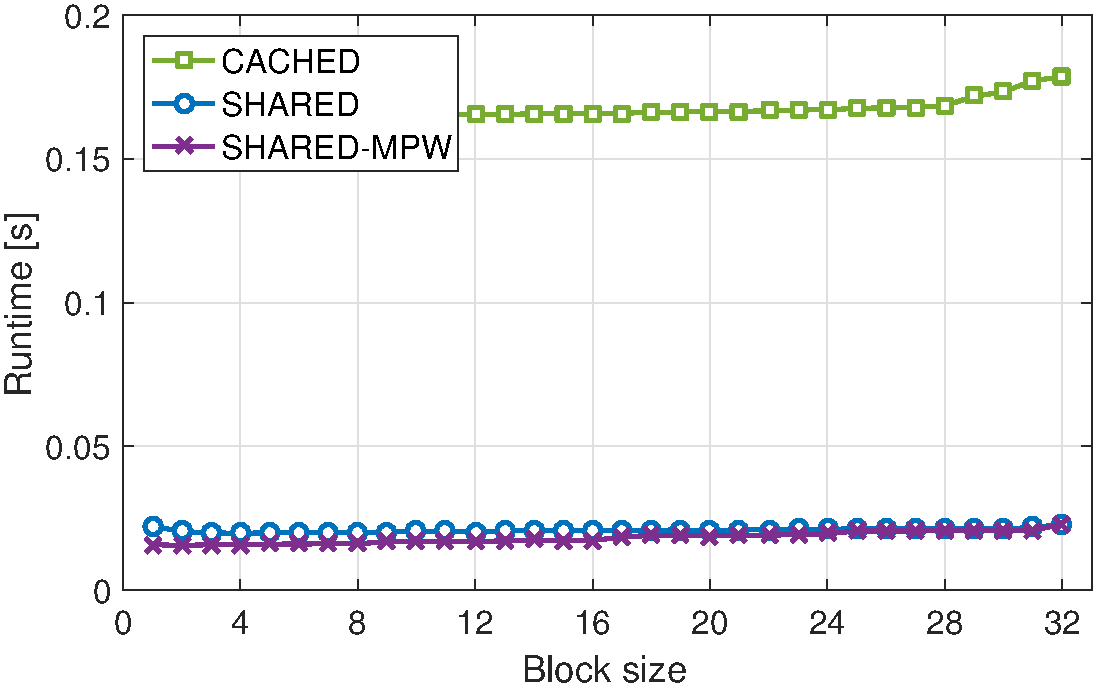
\includegraphics[width=.46\columnwidth]{plots/ARR_bjp_setup_bs_d_P100.pdf}\\
\hline
\multicolumn{2}{c}{Tridiagonal structure}\\
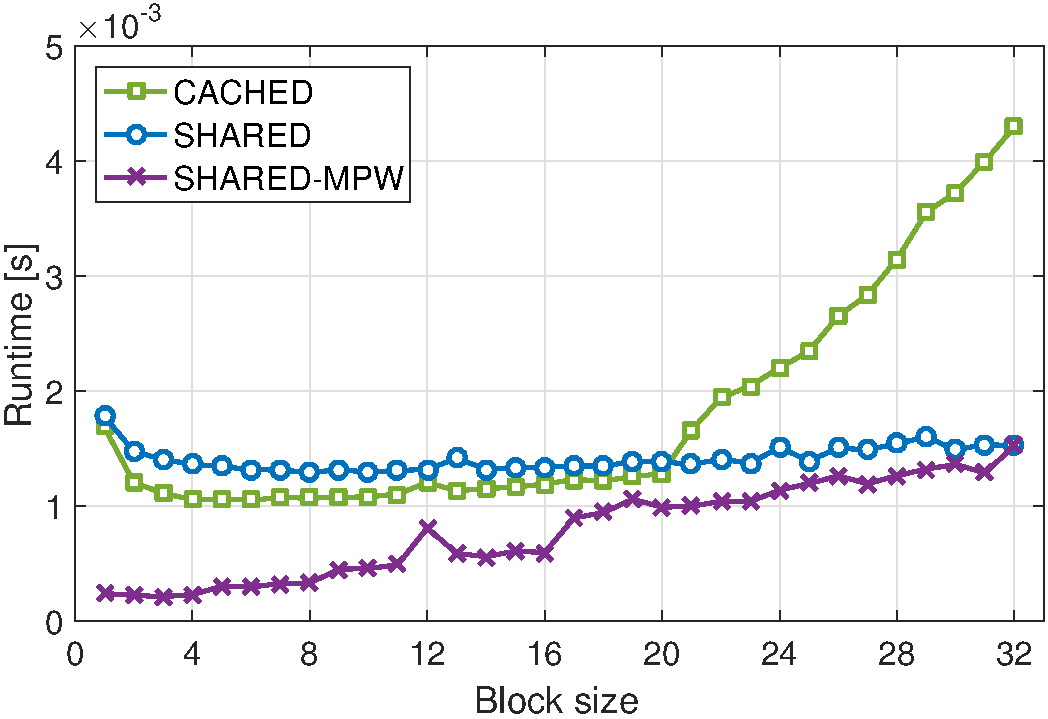
\includegraphics[width=.46\columnwidth]{plots/TDG_bjp_setup_bs_d_K40.pdf}
&
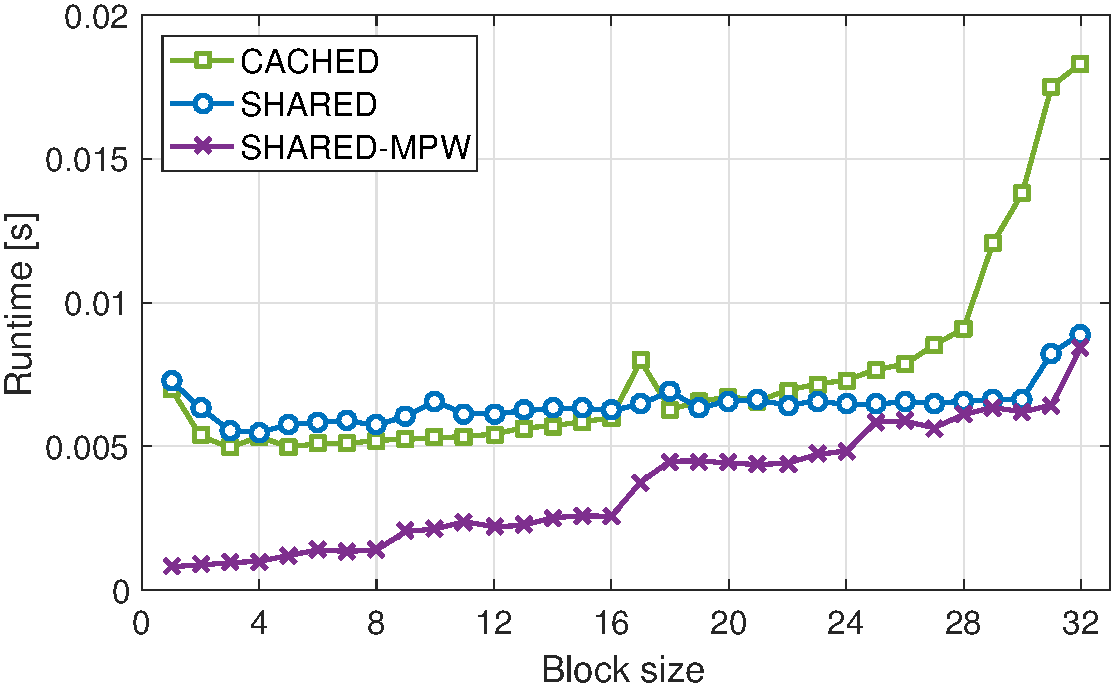
\includegraphics[width=.46\columnwidth]{plots/TDG_bjp_setup_bs_d_P100.pdf}\\
\hline
\multicolumn{2}{c}{Random block structure}\\
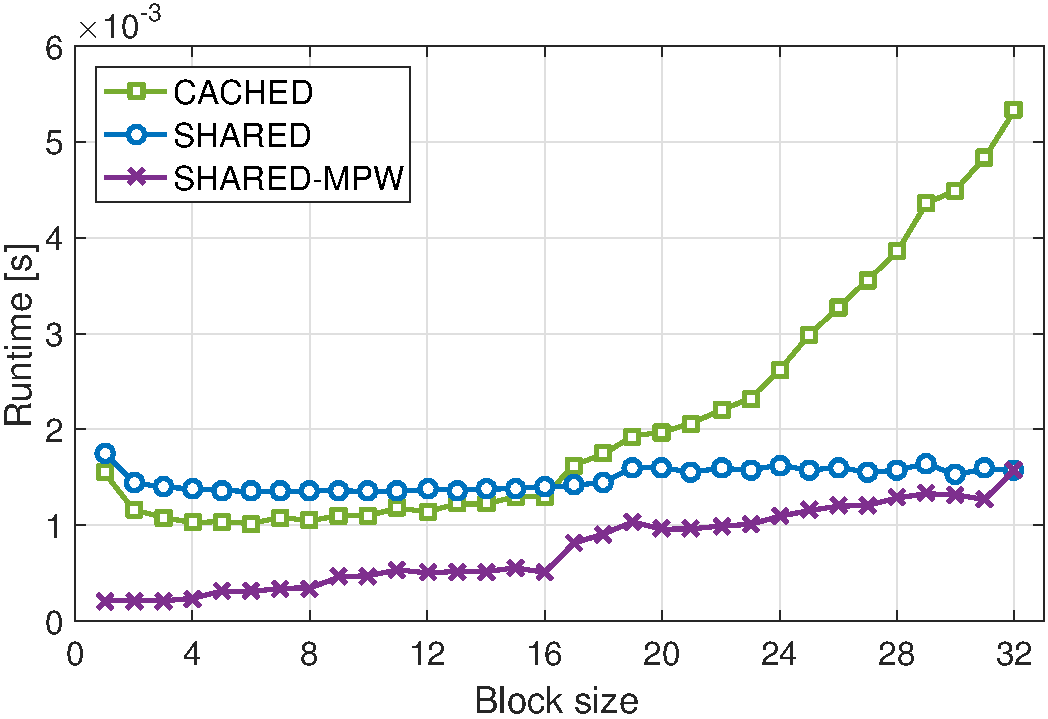
\includegraphics[width=.46\columnwidth]{plots/RND_bjp_setup_bs_d_K40.pdf}
&
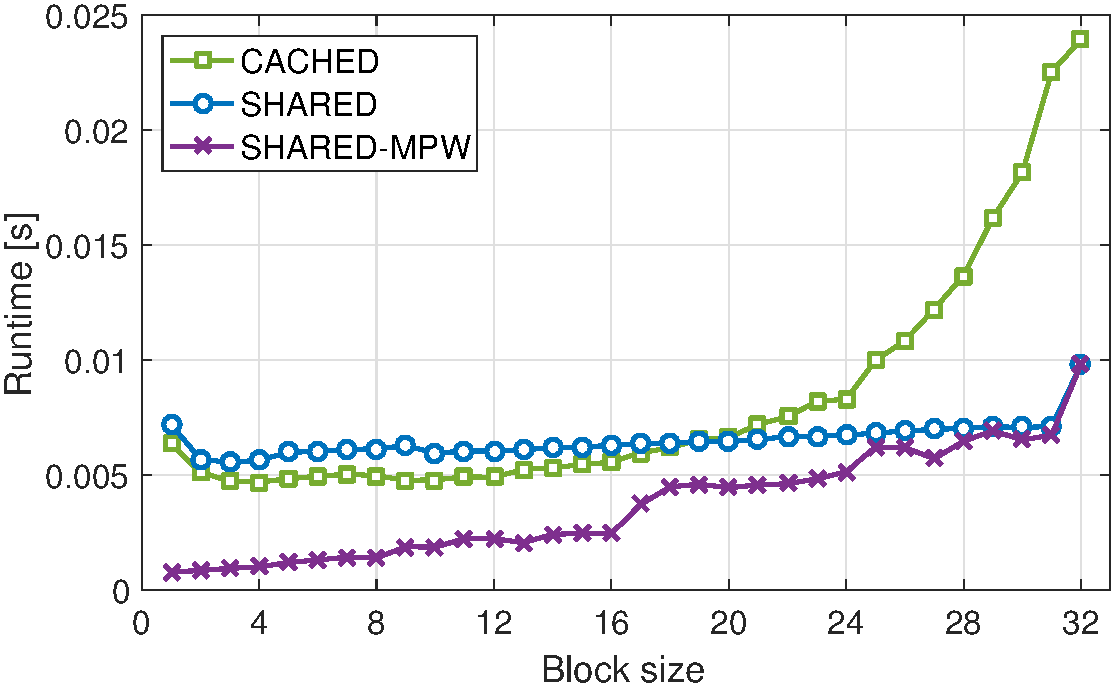
\includegraphics[width=.46\columnwidth]{plots/RND_bjp_setup_bs_d_P100.pdf}\\
\hline
\multicolumn{2}{c}{Laplace structure}\\
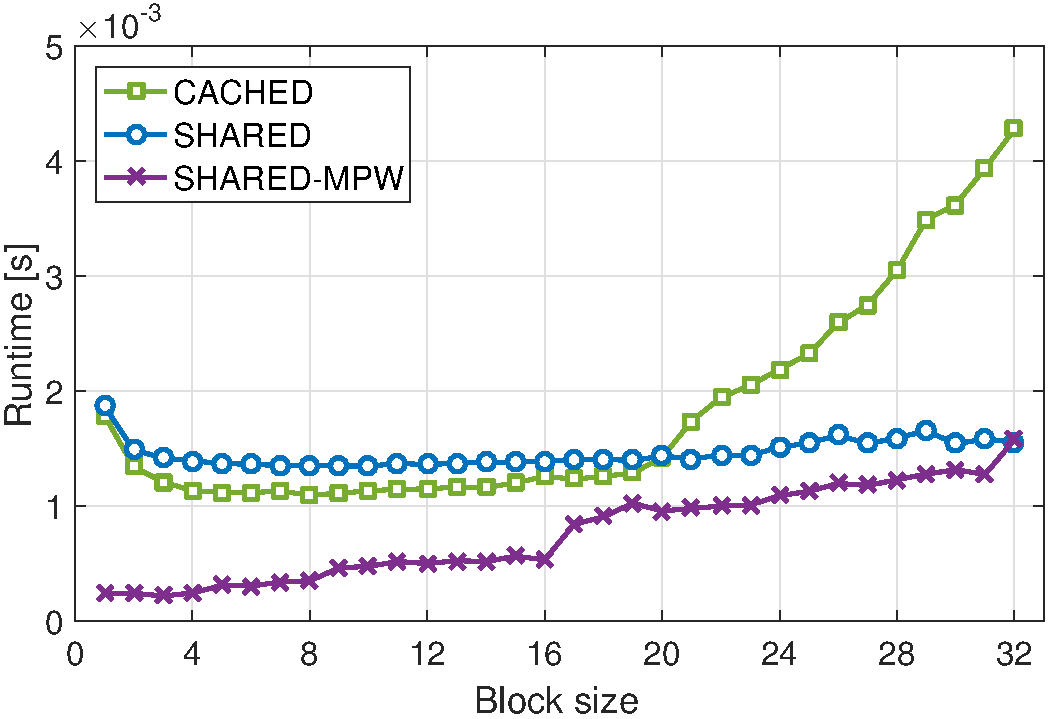
\includegraphics[width=.46\columnwidth]{plots/LAP_bjp_setup_bs_d_K40.pdf}
&
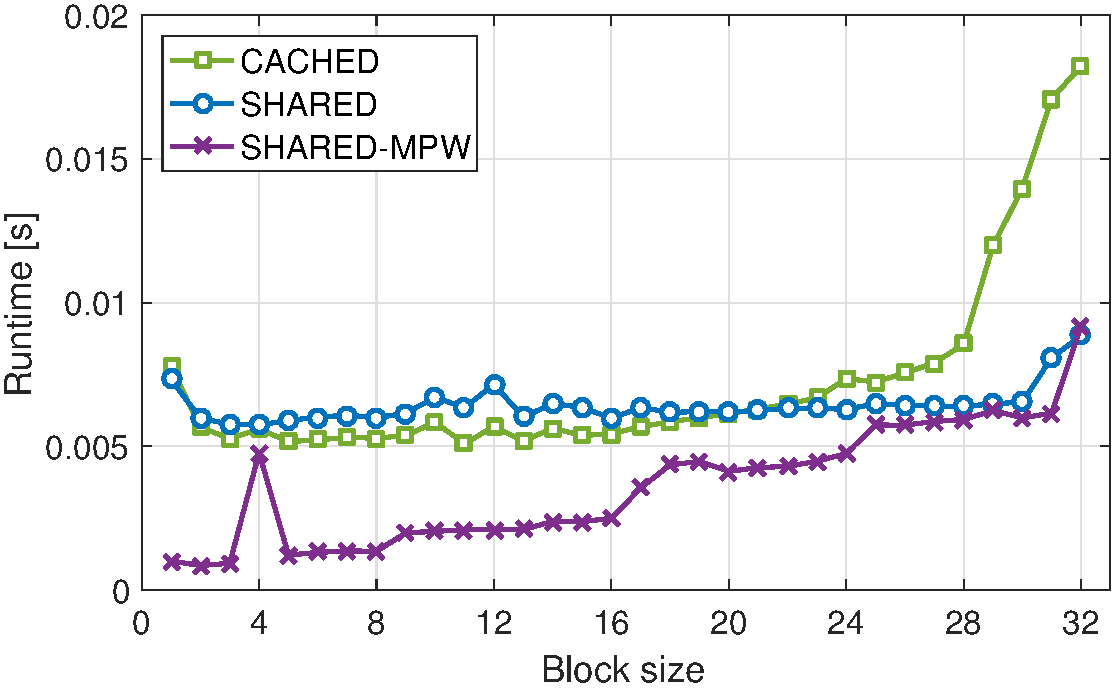
\includegraphics[width=.46\columnwidth]{plots/LAP_bjp_setup_bs_d_P100.pdf}\\
\end{tabular}
}
\end{center}
\caption{
Block-Jacobi generation time for increasing block sizes and nonzero distributions
from top to bottom: arrow, tridiagonal, random block and Laplace.
}
\label{fig:block-jacobi-runtime}
\end{figure*}

Because the performance of the extraction strategies depends on the structure of the
problem matrix, we consider four nonzero distributions that are characteristic
in sparse linear algebra. In Figure~\ref{fig:sparsityplots}, the arrow
	structure presents all nonzero entries on the (main) diagonal plus the last
row/column of the matrix. In contrast, in the tridiagonal structure all
nonzeros lie on the diagonal plus the diagonal immediately above/below it. These
two structures are interesting, because they share the same nonzero count but exhibit
different nonzero distributions. The other two examples correspond to a 
random block-diagonal matrix structure with nonzeros only in the
diagonal blocks. The Laplace structure arises from the five-point
stencil discretization of the Laplace equation.

\begin{figure*}
\begin{center}
{\scriptsize
\begin{tabular}{cc}
\hline
Block size 4 & Block size 8\\
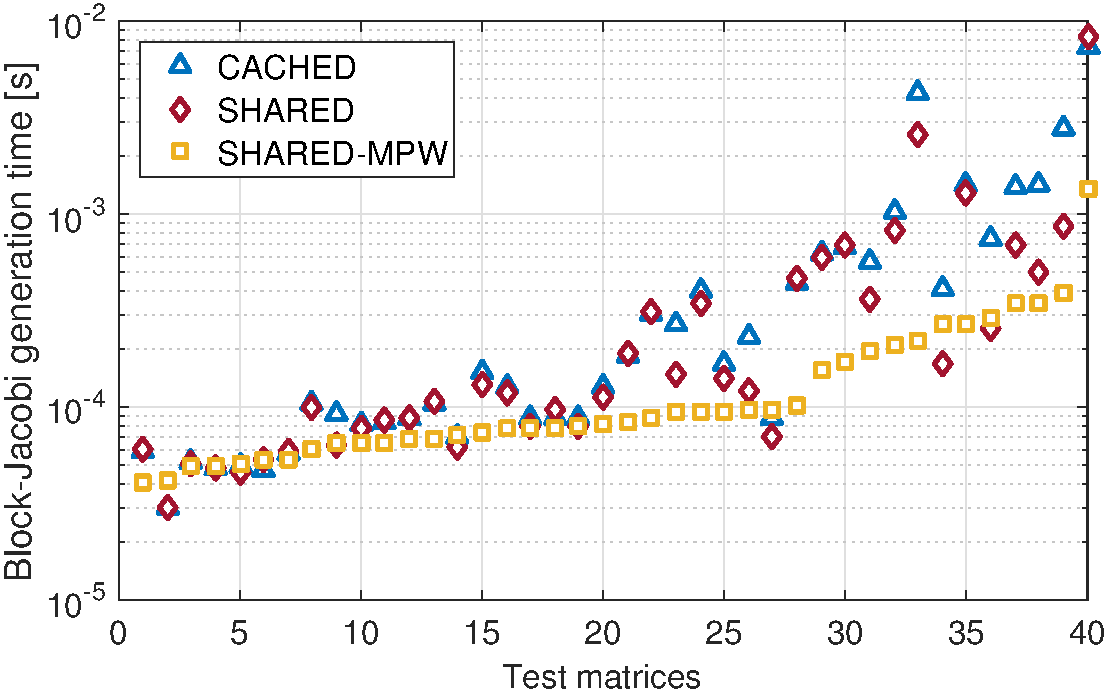
\includegraphics[width=.46\columnwidth]{plots/BJ_generation_time_4.pdf}&
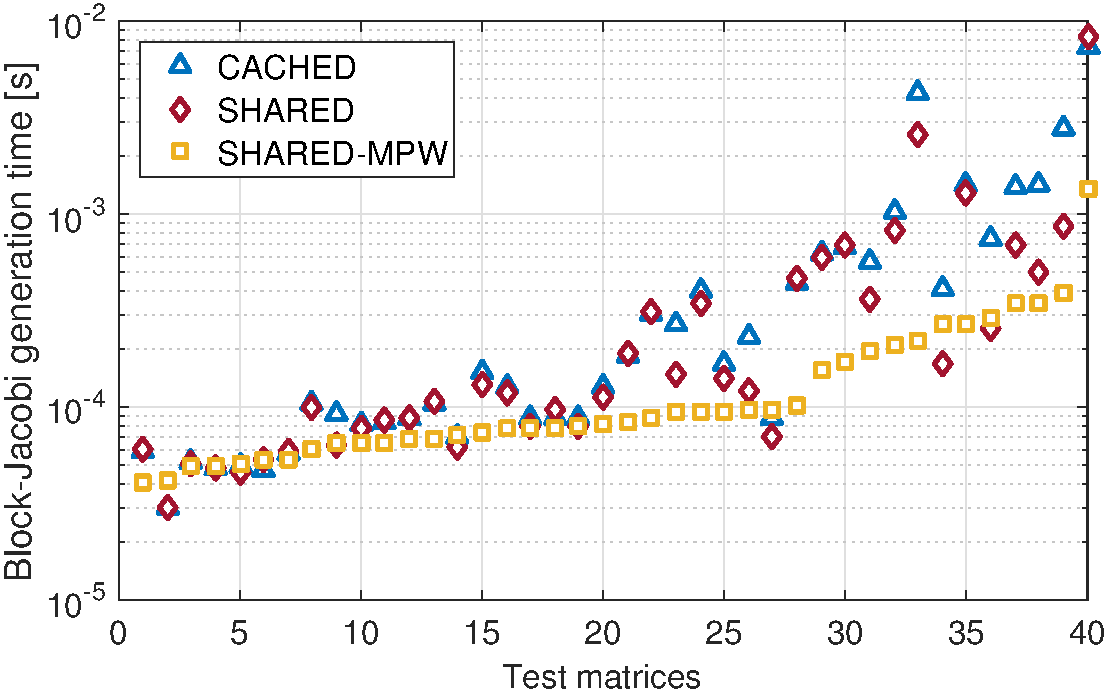
\includegraphics[width=.46\columnwidth]{plots/BJ_generation_time_8.pdf}\\
\hline
Block size 12 & Block size 16\\
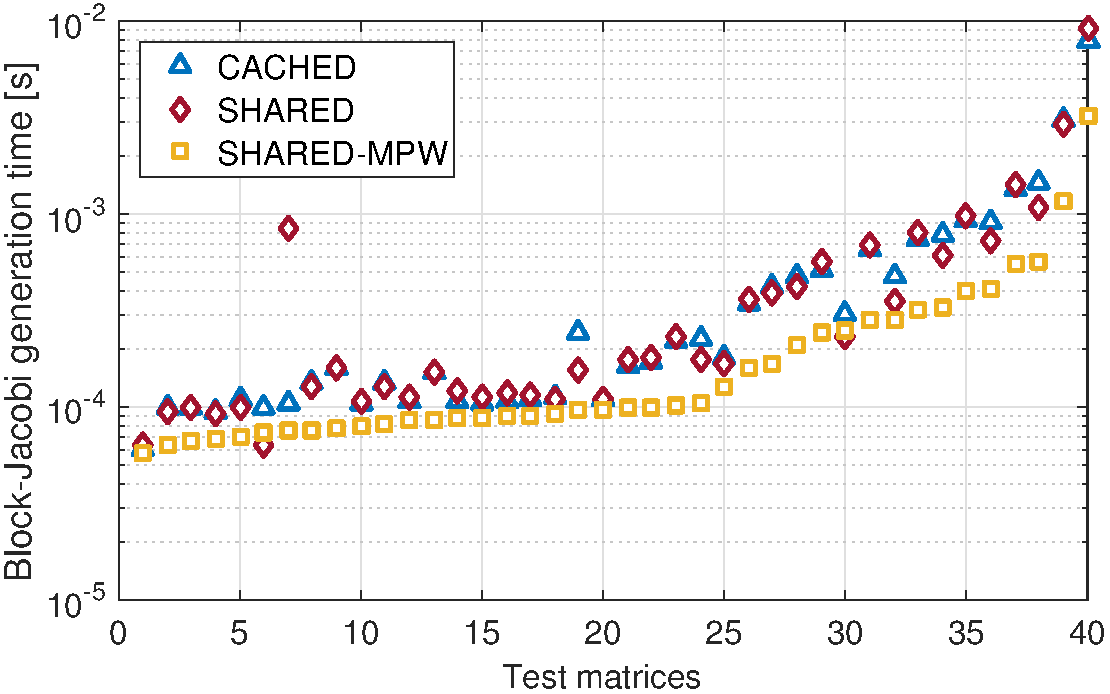
\includegraphics[width=.46\columnwidth]{plots/BJ_generation_time_12.pdf}&
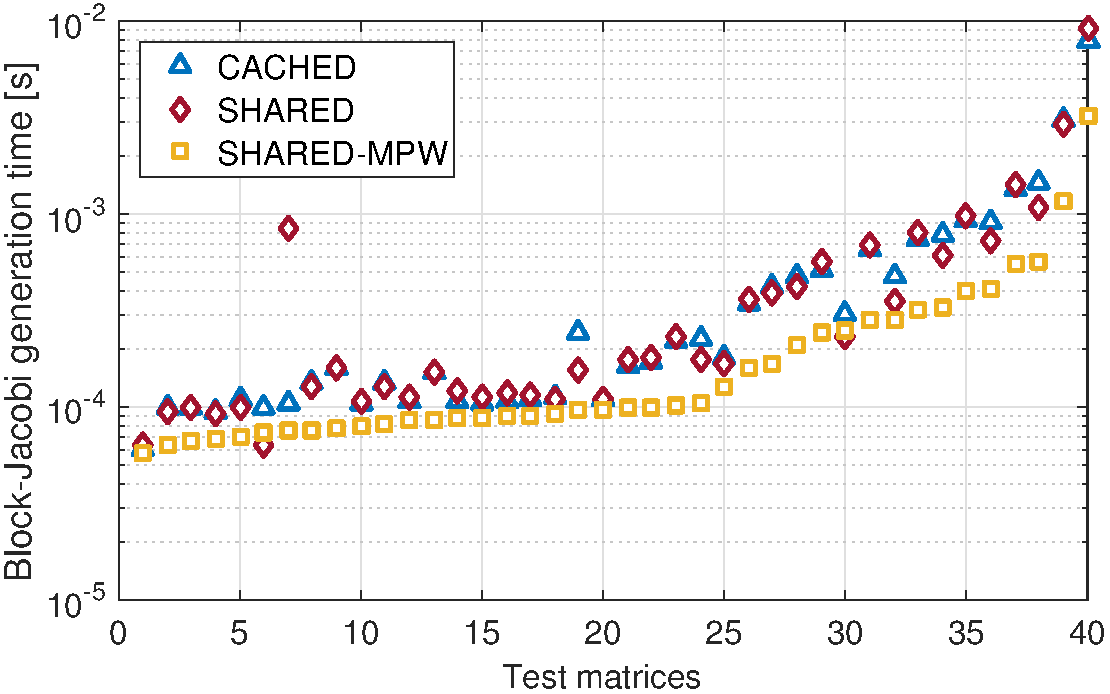
\includegraphics[width=.46\columnwidth]{plots/BJ_generation_time_16.pdf}\\
\hline
Block size 24 & Block size 32\\
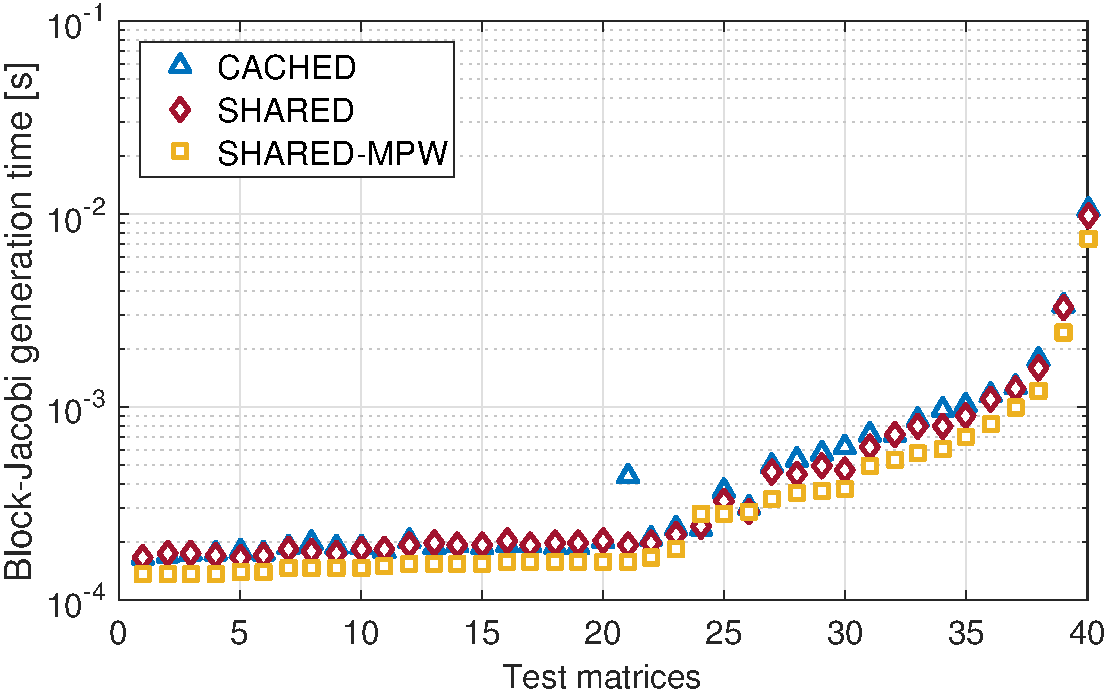
\includegraphics[width=.46\columnwidth]{plots/BJ_generation_time_24.pdf}&
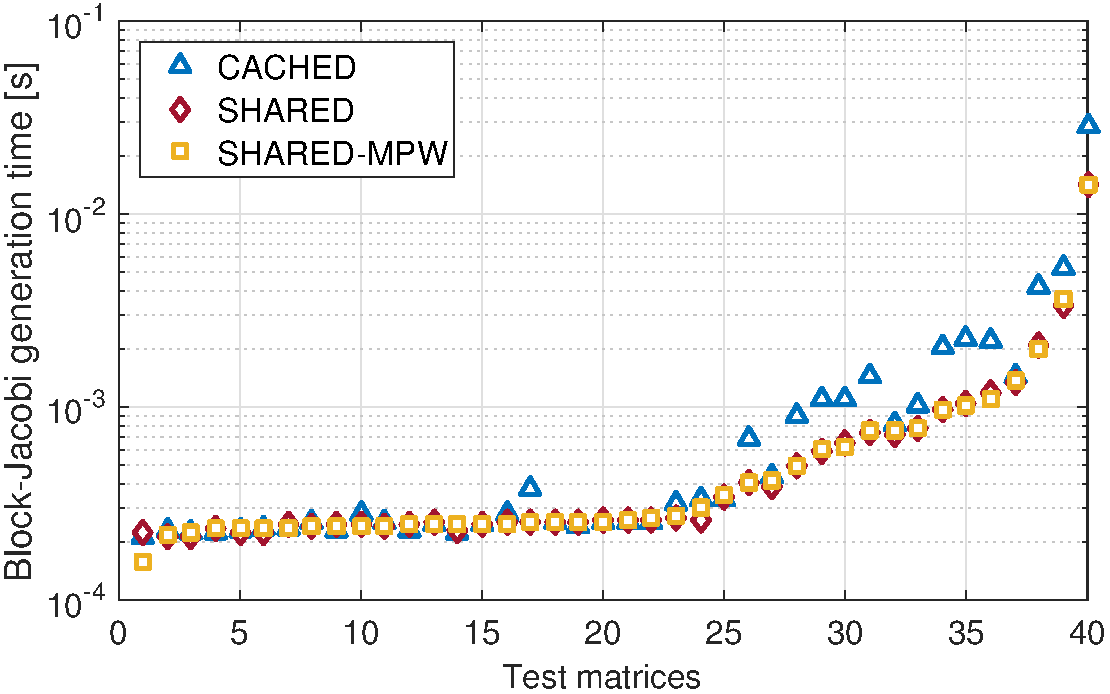
\includegraphics[width=.46\columnwidth]{plots/BJ_generation_time_32.pdf}\\
\end{tabular}
}
\end{center}
\caption{
Block-Jacobi generation time on NVIDIA P100
for a set of matrices taken from the SuiteSparse sparse matrix collection and varied 
block sizes: 4, 8, 12, 16, 24 and 32.
}
\label{fig:block-jacobi-suitsparse}
\end{figure*}


In Figure~\ref{fig:block-jacobi-runtime}, we report the total execution time of
the three block-Jacobi generation strategies applied to the four matrix
structures. In this experiment, we fix the size of the matrix to 1,000,000 and
increase the size of the diagonal blocks from 1 to 32.

For the arrow sparsity structure, the {\sc shared} strategy is much faster than
its {\sc cached} counterpart; see results in the first row of
Figure~\ref{fig:block-jacobi-runtime}. This result was expected because the arrow nonzero
pattern contains a single dense row, which results in dramatic load imbalance if
each row is traversed by a single thread, as is the case for {\sc cached}. The
{\sc shared} alternative uses all threads of the warp to traverse this row,
which alleviates the load imbalance and ensures coalescent access. For the other
cases, the impact of non-coalescent memory access featured by {\sc cached} is
small as long as we consider small block sizes. This is because, for small
blocks, only a few threads in each warp read data, which results in a reduced number
of memory requests. Conversely, for large block sizes, the increase in memory
requests impairs performance. Both strategies based on shared extraction
eliminate load imbalance and non-coalescent memory access. Nonetheless, the
reduced number of idle threads makes the {\sc shared-mpw} version the overall
winner.

We now asses the performance of the extraction routines for a set of test
matrices from the SuiteSparse matrix collection. For brevity, we display the
results for the P100 GPU only. The selected test matrices are listed along with
some key properties in Table~\ref{tab:idr4comparison}. In
Figure~\ref{fig:block-jacobi-suitsparse}, we report the runtime of the
block-Jacobi preconditioner generation for different block sizes. In these
tests, the block sizes only correspond to an upper bound, and the blocks are
identified via supervariable blocking. Also, some blocks can be smaller to better
reflect the block structure of the problem matrix~\cite{chow-scott-2016}. We
again identify {\sc shared-mpw} as the overall winner.


\begin{figure*}
\begin{center}
\begin{tabular}{cc}
K40 & P100\\
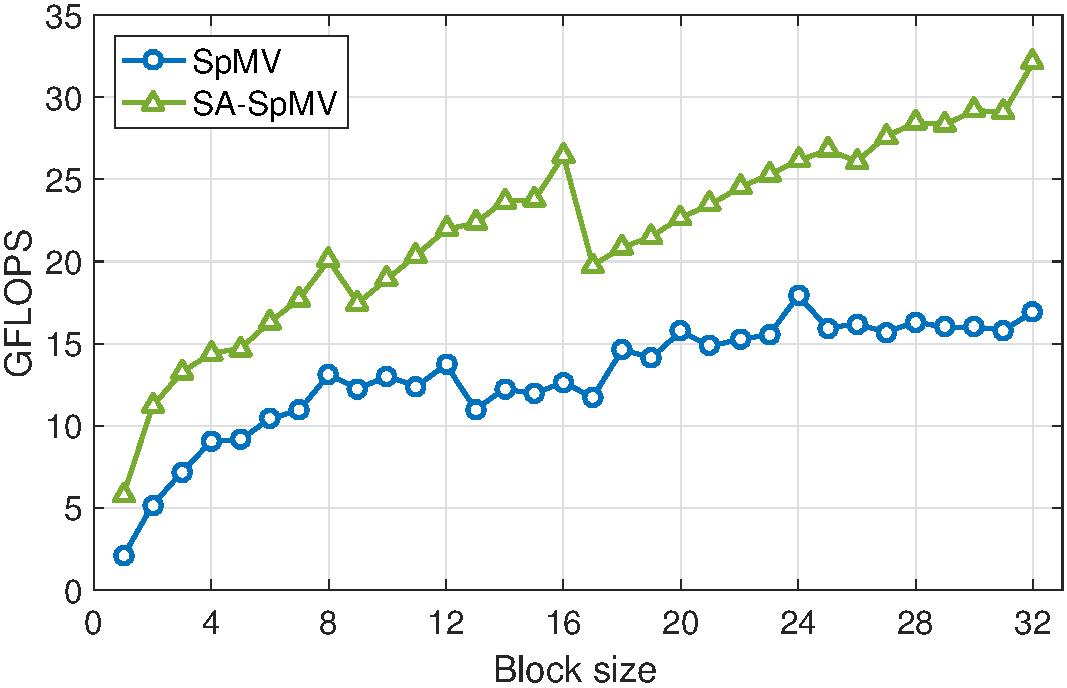
\includegraphics[width=.46\columnwidth]{plots/bjp_apply_bs_d_K40.pdf}
&
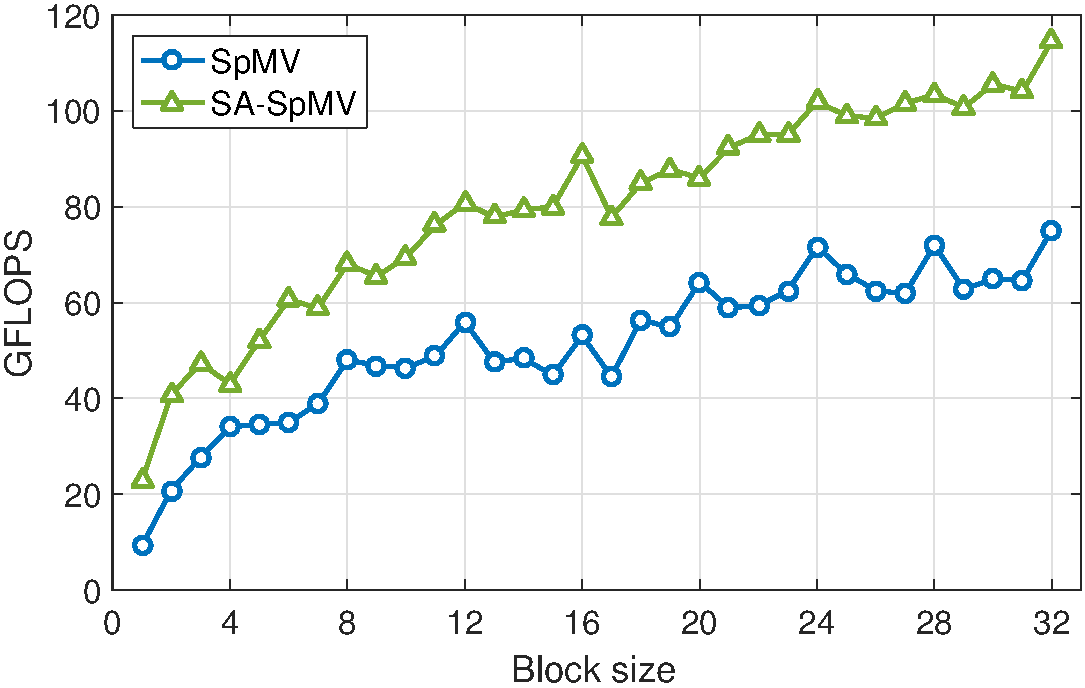
\includegraphics[width=.46\columnwidth]{plots/bjp_apply_bs_d_P100.pdf}
\end{tabular}
\end{center}
\caption{
Performance comparison of the block-Jacobi preconditioner application.
{\sc spmv} is the generic sparse matrix-vector product routine
from~\cite{Anzt:2017:BGE:3026937.3026940}.
{\sc sa-spmv} is the specialized batched {\sc gemv}--based kernel developed as part of this work.  
}
\label{fig:precappl}
\end{figure*}


\subsection{Block-Jacobi application}


In an iterative solver setting, the efficiency of a preconditioner depends on
the overhead of generating the preconditioner and, to even a larger extent, on
the cost of applying it during the iterative solution process.

In Figure~\ref{fig:precappl}, we assess the performance of the preconditioner
application using a generic {\sc spmv} kernel proposed
in~\cite{Anzt:2017:BGE:3026937.3026940} versus our structure-aware {\sc spmv}
({\sc sa-spmv}) introduced in Section~\ref{sec:precapply}. On both architectures,
{\sc sa-spmv} outperforms the initial {\sc spmv} kernel for the preconditioner
application. For a block size of 32, this routine achieves about 32~gigaFLOPS on the K40
architecture, and around 80~gigaFLOPS on the P100 architecture. Local performance peaks
can be identified for block sizes 8 and 16.

\subsection{Convergence in the context of an iterative solver}
\begin{figure*}
\begin{center}
\begin{tabular}{c}
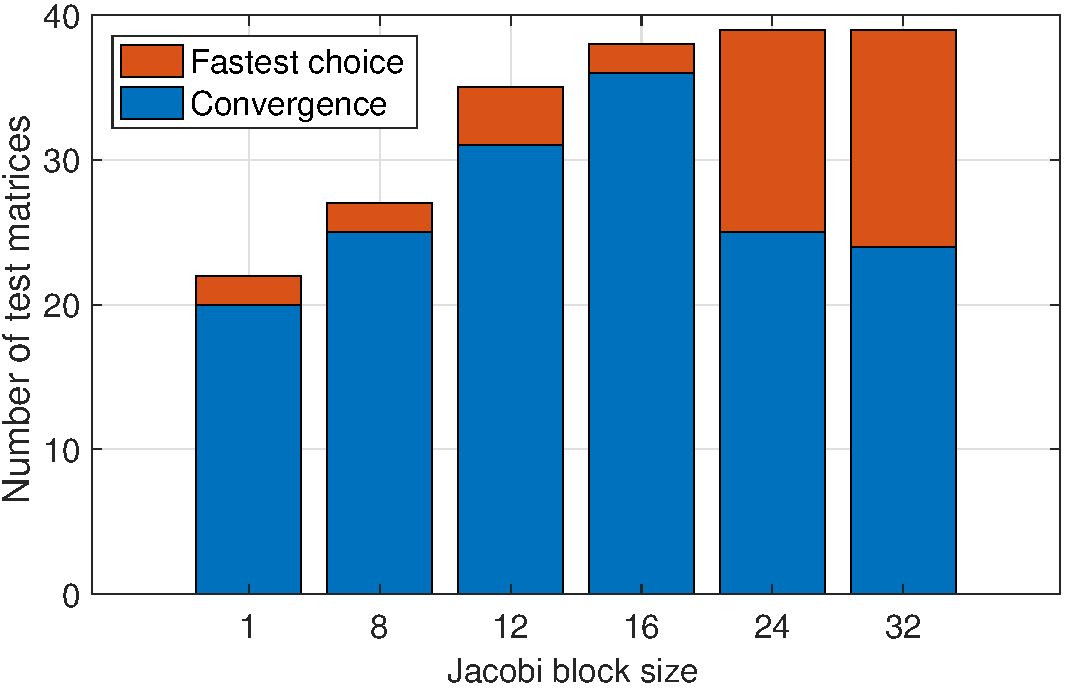
\includegraphics[width=.46\columnwidth]{plots/solverperformance_bs.pdf}
\end{tabular}
\end{center}
\caption{
IDR(4) convergence and performance comparison for different block sizes used in the block-Jacobi preconditioner. 
The problem matrices are listed along with key characteristics in Table~\ref{tab:idr4comparison}.
}
\label{fig:solverperformance}
\end{figure*}

Table~\ref{tab:idr4comparison} in the appendix details the convergence rate and
execution time of an IDR(4) iterative solver~\cite{idr1} enhanced with either a
scalar-Jacobi preconditioner or a block-Jacobi preconditioner for the selected
cases from the SuiteSparse collection. The execution time includes both the
preconditioner generation and the iterative solver execution. 
Detailed analysis reveals that in 88\% of the tests, the preconditioner setup
accounts for less than 1\% of the total execution time. In all other cases, the
block-inverse generation accounts for less than 5\%.
We combine the best
kernels for the distinct preconditioner building blocks, i.e., {\tt SHARED-MPW},
{\tt BGJE-MPW}, and {\tt SA-SPMV}. Other kernels are taken from the MAGMA-sparse
open-source software package~\cite{magma}. The IDR method~\cite{idr} is among the 
most robust Krylov solvers~\cite{ashes2016}. The GPU-implementation of IDR available in
MAGMA-sparse has been proven to achieve performance close to the hardware-imposed
bounds~\cite{ijhpca2016}. For brevity, we run these tests on the newer P100
architecture only. We start the iterative solution process with an initial guess, 
$x_0=0$, solve for a right-hand side composed of random values in the interval
$[0,1]$, and stop the iteration process once the relative residual norm has
decreased by nine orders of magnitude. We allow for up to 50,000 iterations of
the IDR(4) solver. In Figure~\ref{fig:solverperformance}, we summarize the
results showing for how many problems a certain configuration was the best
choice (i.e., provided the fastest time to solution), and for how many problems
a certain configuration was ``successful'' (concretely, reduced the relative
residual norm by nine orders of magnitude within the limit of 50,000
iterations).


The results reveal that the scalar version of Jacobi fails to sufficiently
improve the convergence of IDR(4) for a significant fraction of the test
matrices.
For the test matrices where IDR(4) preconditioned with the scalar Jacobi
converges, the faster convergence obtained from using a block-Jacobi
preconditioner typically compensates for the higher costs of preconditioner
setup and application.
In Figure~\ref{fig:solverperformance-detailed}, we offer a
head-to-head comparison of different block-size bounds for the
block-Jacobi preconditioner used in IDR(4).
The orange area in the plot at position ``row Jacobi($x$) vs. column 
Jacobi($y$)'' 
visualizes the number of matrices for which IDR(4) preconditioned with 
block-Jacobi of block size $x$ converged, while it failed to converge with block size $y$. 
The opposite scenario, where block size $y$ converged
but block size $x$ did not, is shown in green. Finally, the yellow area 
represents the
number of matrices for which both methods converged---the area to the right of 
the center represents cases where block size $y$ converges faster, while the
area left of the center represents cases where block size $x$ converges faster. 
The results suggest that adopting a larger block size usually leads to a more robust solver
(i.e., convergence is achieved for a larger number of problems), and that a
larger block size also improves the overall time-to-solution performance.
However, in order to obtain the optimal performance for a specific problem, the
block size should be tuned to the underlying block structure of the problem.

Overall, the results presented in this subsection offer strong evidence that the
routines we developed
provide an efficient approach to generating and applying a block-Jacobi
preconditioner.

\begin{landscape}

\begin{figure}
\begin{center}
{\scriptsize
\begin{tabular}{c|cccccc}
& \textbf{Jacobi(1)}&\textbf{Jacobi(8)}&\textbf{Jacobi(12)}&\textbf{Jacobi(16)}&\textbf{Jacobi(24)}&\textbf{Jacobi(32)}\\
\hline
\parbox[t]{2mm}{\multirow{1}{*}{\rotatebox[origin=r]{90}{\textbf{
    Jacobi(32)\hspace*{1.08cm}
    Jacobi(24)\hspace*{1.08cm}
    Jacobi(16)\hspace*{1.08cm}
    Jacobi(12)\hspace*{1.08cm}
    Jacobi(8)\hspace*{1.2cm}
    Jacobi(1)\hspace*{.5cm}}}}
}
\\

&
 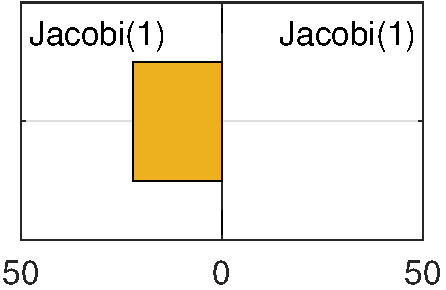
\includegraphics[width=.135\columnwidth]{plots/Jacobi(1)_vs_Jacobi(1).pdf}
&
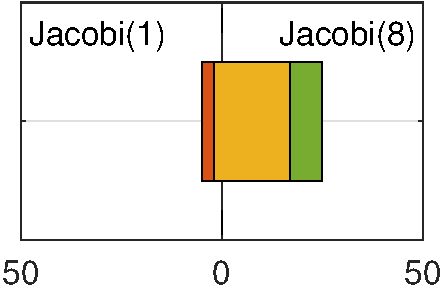
\includegraphics[width=.135\columnwidth]{plots/Jacobi(1)_vs_Jacobi(8).pdf}
&
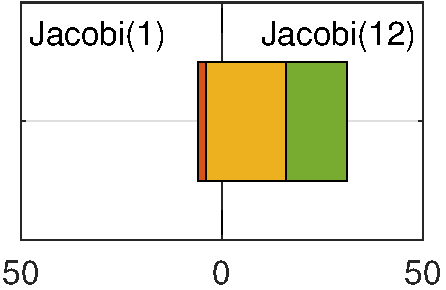
\includegraphics[width=.135\columnwidth]{plots/Jacobi(1)_vs_Jacobi(12).pdf}
&
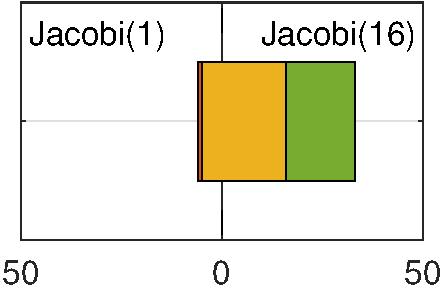
\includegraphics[width=.135\columnwidth]{plots/Jacobi(1)_vs_Jacobi(16).pdf}
&
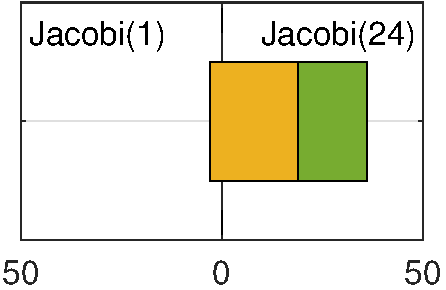
\includegraphics[width=.135\columnwidth]{plots/Jacobi(1)_vs_Jacobi(24).pdf}
&
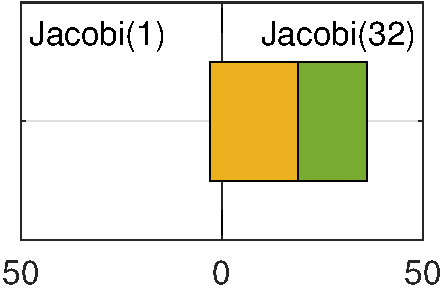
\includegraphics[width=.135\columnwidth]{plots/Jacobi(1)_vs_Jacobi(32).pdf}
\\
&
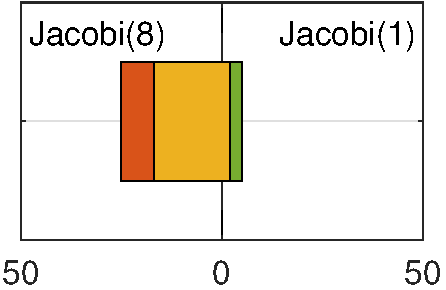
\includegraphics[width=.135\columnwidth]{plots/Jacobi(8)_vs_Jacobi(1).pdf}
&
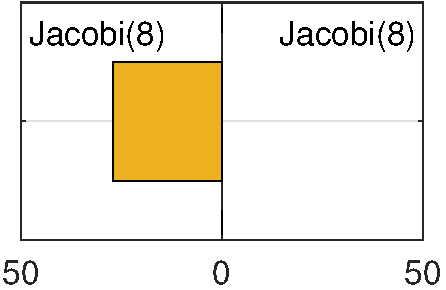
\includegraphics[width=.135\columnwidth]{plots/Jacobi(8)_vs_Jacobi(8).pdf}
&
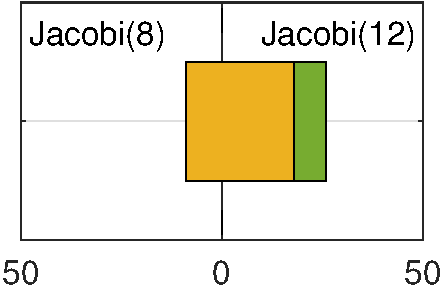
\includegraphics[width=.135\columnwidth]{plots/Jacobi(8)_vs_Jacobi(12).pdf}
&
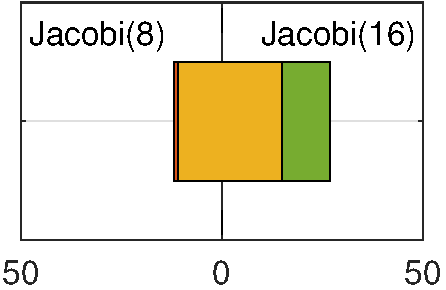
\includegraphics[width=.135\columnwidth]{plots/Jacobi(8)_vs_Jacobi(16).pdf}
&
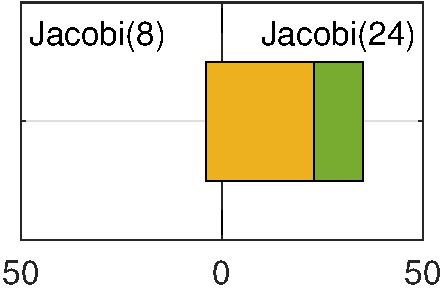
\includegraphics[width=.135\columnwidth]{plots/Jacobi(8)_vs_Jacobi(24).pdf}
&
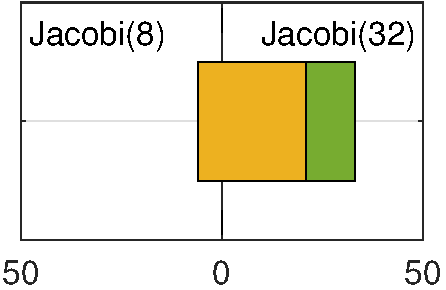
\includegraphics[width=.135\columnwidth]{plots/Jacobi(8)_vs_Jacobi(32).pdf}
\\
&
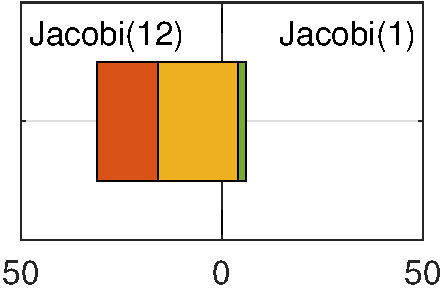
\includegraphics[width=.135\columnwidth]{plots/Jacobi(12)_vs_Jacobi(1).pdf}
&
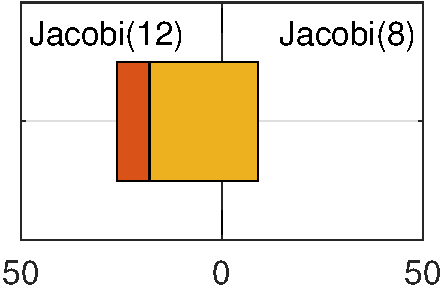
\includegraphics[width=.135\columnwidth]{plots/Jacobi(12)_vs_Jacobi(8).pdf}
&
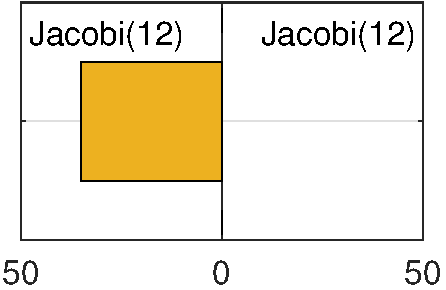
\includegraphics[width=.135\columnwidth]{plots/Jacobi(12)_vs_Jacobi(12).pdf}
&
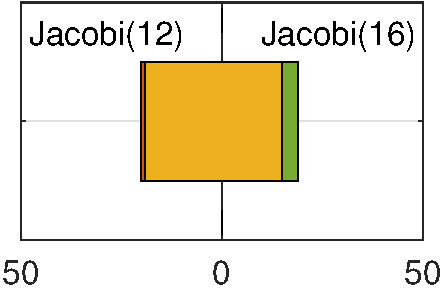
\includegraphics[width=.135\columnwidth]{plots/Jacobi(12)_vs_Jacobi(16).pdf}
&
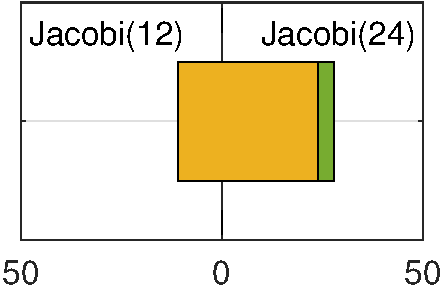
\includegraphics[width=.135\columnwidth]{plots/Jacobi(12)_vs_Jacobi(24).pdf}
&
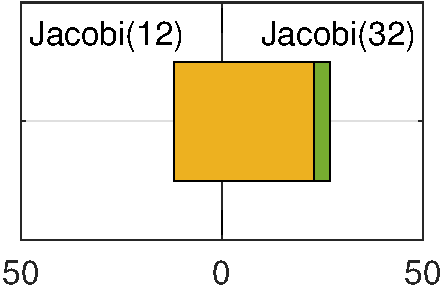
\includegraphics[width=.135\columnwidth]{plots/Jacobi(12)_vs_Jacobi(32).pdf}
\\
&
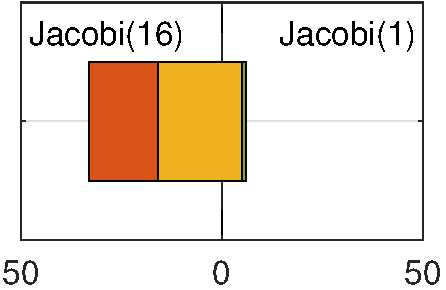
\includegraphics[width=.135\columnwidth]{plots/Jacobi(16)_vs_Jacobi(1).pdf}
&
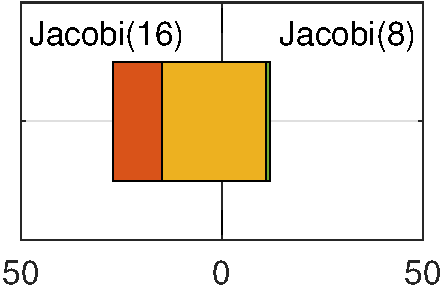
\includegraphics[width=.135\columnwidth]{plots/Jacobi(16)_vs_Jacobi(8).pdf}
&
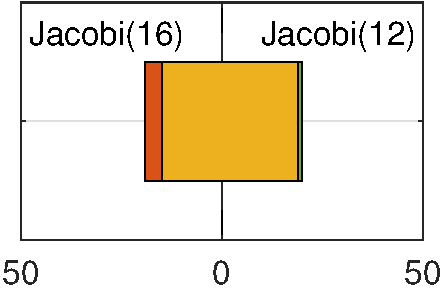
\includegraphics[width=.135\columnwidth]{plots/Jacobi(16)_vs_Jacobi(12).pdf}
&
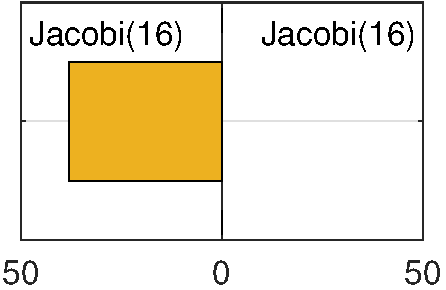
\includegraphics[width=.135\columnwidth]{plots/Jacobi(16)_vs_Jacobi(16).pdf}
&
\includegraphics[width=.135\columnwidth]{plots/Jacobi(16)_vs_Jacobi(24).pdf}
&
\includegraphics[width=.135\columnwidth]{plots/Jacobi(16)_vs_Jacobi(32).pdf}
\\
&
\includegraphics[width=.135\columnwidth]{plots/Jacobi(24)_vs_Jacobi(1).pdf}
&
\includegraphics[width=.135\columnwidth]{plots/Jacobi(24)_vs_Jacobi(8).pdf}
&
\includegraphics[width=.135\columnwidth]{plots/Jacobi(24)_vs_Jacobi(12).pdf}
&
\includegraphics[width=.135\columnwidth]{plots/Jacobi(24)_vs_Jacobi(16).pdf}
&
\includegraphics[width=.135\columnwidth]{plots/Jacobi(24)_vs_Jacobi(24).pdf}
&
\includegraphics[width=.135\columnwidth]{plots/Jacobi(24)_vs_Jacobi(32).pdf}
\\
&
\includegraphics[width=.135\columnwidth]{plots/Jacobi(32)_vs_Jacobi(1).pdf}
&
\includegraphics[width=.135\columnwidth]{plots/Jacobi(32)_vs_Jacobi(8).pdf}
&
\includegraphics[width=.135\columnwidth]{plots/Jacobi(32)_vs_Jacobi(12).pdf}
&
\includegraphics[width=.135\columnwidth]{plots/Jacobi(32)_vs_Jacobi(16).pdf}
&
\includegraphics[width=.135\columnwidth]{plots/Jacobi(32)_vs_Jacobi(24).pdf}
&
 \includegraphics[width=.135\columnwidth]{plots/Jacobi(32)_vs_Jacobi(32).pdf}
\\
\end{tabular}
}
\end{center}
\caption{
Detailed comparison of IDR(4) enhanced with block Jacobi
using different block sizes.
}
\label{fig:solverperformance-detailed}
\end{figure}

\end{landscape}
